\chapter{Calculation of Elastic Parameters of alpha-uranium}\label{appen_elalpha}

In this appendix, we will discuss the stress-strain relationships that was used to calculated the nine independent elastic constants of \textalpha-uranium. The base-centered orthorhombic phase of uranium has three lattice parameters $a$, $b$, and $c$, with the Bravais lattice matrix.

\begin{equation}\label{eq_lattic_alphaU}
\mathbf{R} = \begin{pmatrix}
			\frac{a}{2} & -\frac{b}{2} & 0 \\
			\frac{a}{2} & \frac{b}{2} & 0 \\
			0			&    0        & c 
			\end{pmatrix}
\end{equation}

Applying a small strain to the equilibrium lattice changes the total energy, and from this information, the elastic parameters are deduced. The elastic parameters are identified as proportional to the second order coefficient in a polynomial fit of the total energy as a function of the distortion parameter $\delta$~\cite{wallace1998thermodynamics}. The distortion of lattice vector follows the rule $\mathbf{R'}=\mathbf{RD}$. Here $\mathbf{R'}$ is a matrix containing the components of the distorted lattice vectors and $\mathbf{D}$ is the symmetric distortion matrix.



The internal energy of a crystal under strain, $\delta$, can be Taylor expanded in powers of the strain tensor with respect to initial energy of the unstrained crystal in the following way:
	\begin{equation}
	\label{eq_taylor_el}
	E(V,\delta) = E(V_0,0) + V_0 \left ( \sum_i \tau_i \xi_i d_1 + 1/2 \sum_{ij} c_{ij} \delta_i \xi_i \delta_j \xi_j \right ) + O(\delta^3) 
	\end{equation}

The unstrained volume is $V_0$, and $E(V_0,0)$ is the energy of the unstrained system. The Voight notation has been used in the above equation, i.e. $xx$, $yy$, $zz$, $yz$, $xz$ and $xy$ are replaced with 1--6. Here $yz$, $xz$ and $xy$ are equal to $zy$, $zx$ and $yx$ and for this reason $\xi_i$ is equal to 1 for $i=1$, $2$, and $3$ and $2$ for $i=4$, $5$ and $6$. $\tau_i$ is a component of stress tensor. The first three elastic constants $c_{11}$, $c_{22}$ and $c_{33}$ are obtained form the following distortions:
\begin{equation}
\label{eq_D1}
	D_1 =  \begin{pmatrix}
						1+\delta & 0 & 0 \\
						0 & 1 & 0 \\
						0 & 0 & 1 \\
						\end{pmatrix}
\end{equation}

\begin{equation}
\label{eq_D2}
	D_2 = \begin{pmatrix}
						1 & 0 & 0 \\
						0 & 1+\delta & 0 \\
						0 & 0 & 1 \\
					\end{pmatrix}
\end{equation}

\begin{equation}
\label{eq_D3}
D_3 =  \begin{pmatrix}
						1 & 0 & 0 \\
						0 & 1 & 0 \\
						0 & 0 & 1+\delta \\
						\end{pmatrix}
\end{equation}

The internal energies for these three distortions can be obtained from 
\begin{equation}
\label{eq_d1d2d3}
E(V,\delta) = E(V_0,0) + V_0\tau_i \delta + \frac{V_0C_{ii}\delta^2}{2}
\end{equation}

The $c_{44}$, $c_{55}$ and $c_{66}$ are related to the distortion equations:
\begin{equation}
\label{eq_D4}
	D_4 = \begin{pmatrix}
						\frac{1}{(1-\delta^2)^{1/3}} & 0 & 0 \\
						0 & \frac{1}{(1-\delta^2)^{1/3}} & \frac{\delta}{(1-\delta^2)^{1/3}} \\
						0 & \frac{\delta}{(1-\delta^2)^{1/3}} & \frac{1}{(1-\delta^2)^{1/3}} \\
						\end{pmatrix}
\end{equation} 

\begin{equation}
\label{eq_D5}
	D_5 =  \begin{pmatrix}
						\frac{1}{(1-\delta^2)^{1/3}} & 0 & \frac{\delta}{(1-\delta^2)^{1/3}} \\
						0 & \frac{1}{(1-\delta^2)^{1/3}} & 0 \\
						\frac{\delta}{(1-\delta^2)^{1/3}} & 0 & \frac{1}{(1-\delta^2)^{1/3}} \\
						\end{pmatrix}
\end{equation}

\begin{equation}\label{eq_D6}
						D_6 = \begin{pmatrix}
						\frac{1}{(1-\delta^2)^{1/3}} & \frac{\delta}{(1-\delta^2)^{1/3}} & 0 \\
						\frac{\delta}{(1-\delta^2)^{1/3}} & \frac{1}{(1-\delta^2)^{1/3}} & 0 \\
						0 & 0 & \frac{1}{(1-\delta^2)^{1/3}} \\
						\end{pmatrix}
\end{equation}	


These three elastic constants can be calculated from the corresponding internal energy:
\begin{equation}
							E(V,\delta) = E(V_0,0) + V_0\tau_i \delta + \frac{V_0C_{ii}\delta^2}{2}
\end{equation}

The last three distortions are:

\begin{equation}\label{eq_D7}
						D_7 = \begin{pmatrix}
						\frac{1+\delta}{(1-\delta^2)^{1/3}} & 0 & 0 \\
						0 & \frac{1-\delta}{(1-\delta^2)^{1/3}} & 0 \\
						0 & 0 & \frac{1}{(1-\delta^2)^{1/3}} \\	
						\end{pmatrix}
\end{equation}			

\begin{equation}\label{eq_D8}
						D_8 =  \begin{pmatrix}
						\frac{1+\delta}{(1-\delta^2)^{1/3}} & 0 & 0 \\
						0 & \frac{1}{(1-\delta^2)^{1/3}} & 0 \\
						0 & 0 & \frac{1-\delta}{(1-\delta^2)^{1/3}} \\
						\end{pmatrix}
\end{equation}	

\begin{equation}\label{eq_D9}
						D_9 = \begin{pmatrix}
						\frac{1}{(1-\delta^2)^{1/3}} & 0 & 0 \\
						0 & \frac{1+\delta}{(1-\delta^2)^{1/3}} & 0 \\
						0 & 0 & \frac{1-\delta}{(1-\delta^2)^{1/3}} \\	
						\end{pmatrix}
\end{equation}

The internal energies related with these three distortions are given by the following equations:
\begin{equation}
E(V,\delta) = E(V_0, 0) + V_0\left [ \tau_1 - \tau_2 \right ] \delta + \frac{1}{2} \left(c_{11} + c_{22} -2c_{12}  \right)\delta^2
\end{equation}

\begin{equation}
E(V,\delta) = E(V_0, 0) + V_0\left [ \tau_1 - \tau_3 \right ] \delta + \frac{1}{2} \left(c_{11} + c_{33} -2c_{13}  \right)\delta^2
\end{equation}

\begin{equation}
E(V,\delta) = E(V_0, 0) + V_0\left [ \tau_2 - \tau_3 \right ] \delta + \frac{1}{2} \left(c_{22} + c_{33} -2c_{23}  \right)\delta^2
\end{equation}
The above equations can be used to calculated the remaining elastic constants $c_{12}$, $c_{13}$, and $c_{23}$. The energy and strain relations are calculated and included in Figure~\ref{fig_D123}, \ref{fig_D456}, and \ref{fig_D789}. 

\begin{figure}
	\centering
	\includegraphics[]{d123_alphaU.eps}
	\caption[Changes in strain energy in $D_1$, $D_2$ and $D_3$]{Changes in the strain energy as a function of strain using distortion matrix~$D_1$~\eqref{eq_D1}, $D_2$~\eqref{eq_D2} and $D_3$~\eqref{eq_D3}.}
	\label{fig_D123}
\end{figure}

\begin{figure}
	\centering
	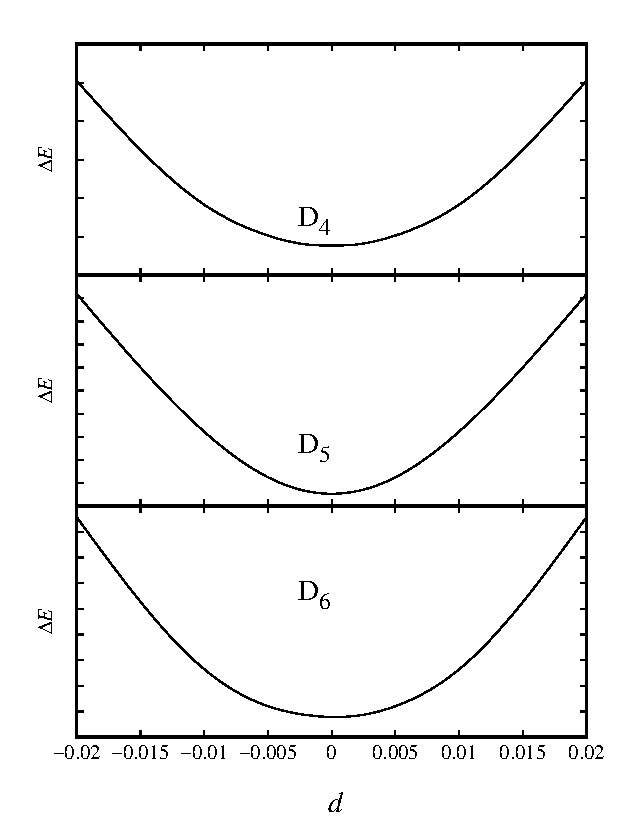
\includegraphics[]{d456_alphaU.eps}
	\caption[Changes in strain energy in $D_4$, $D_5$ and $D_6$]{Changes in the strain energy as a function of strain using distortion matrix~$D_4$~\eqref{eq_D4}, $D_5$~\eqref{eq_D5} and $D_6$~\eqref{eq_D6}.}
	\label{fig_D456}
\end{figure}

\begin{figure}
	\centering
	\includegraphics[]{d789_alphaU.eps}
	\caption[Changes in strain energy in $D_7$, $D_8$ and $D_9$]{Changes in the strain energy as a function of strain using distortion matrix~$D_7$~\eqref{eq_D7}, $D_8$~\eqref{eq_D8} and $D_9$~\eqref{eq_D9}.}
	\label{fig_D789}
\end{figure}



\bibliographystyle{unsrt}
\bibliography{abbreviated,comp}
